%GA: não gostei tanto do nome da section
\section{Health-Related Processes and Services}
\label{sec:results_health_processes_services}

The final set of experiments examines processes in which population mobility interacts with health-related state changes and access to recurring services. Unlike the preceding experiments, where the principal outcomes are population movement, activity fulfillment, or displacement, these scenarios introduce outcomes associated with the evolution of population health states and the ability of service facilities to meet recurring demand.

Two applications are considered. The first examines epidemic contagion and evaluates how changes in transmission intensity, vaccination schedules, and movement restrictions alter the progression of infection. The second examines access to dialysis treatment under service-capacity constraints and disruptions to clinics and supporting infrastructure. The corresponding plugins, state representations, service inputs, and infrastructure dependencies are described in Section~\ref{sec:health_processes_services}.%; the present section focuses on the experimental configurations and the resulting population- and service-level outcomes.

Accordingly, these experiments address three broader questions: (i) how population-level health states evolve when contagion operates together with normal-life mobility; (ii) how configured interventions modify this progression; and (iii) how recurring healthcare demand responds to limitations in service capacity and infrastructure availability. Because the epidemic and dialysis experiments use different populations, spatial representations, simulation horizons, and outcome definitions, quantitative comparisons are performed within each experiment group rather than between them.


\subsection{Experimental Overview}
\label{sec:health_results_overview}

The health-related experiments are organized into two main groups. The epidemic experiments use the neighborhood-level representation of Porto Alegre and extend the normal-life mobility baseline with infection and vaccination states. They first vary the configured infection intensity and subsequently evaluate vaccination and movement-restriction scenarios. These experiments correspond to the configurations originally reported with the publisehd manuscript~\cite{silva2026lodusPop}.

The dialysis experiments instead use the reduced and complete census-sector environments. They examine recurring treatment demand under differences in demand, clinic availability, water-infrastructure dependencies, environmental disruption, recovery, and the spatial distribution of unavailable treatment capacity.

Table~\ref{tbl:health_results_overview} summarizes the principal experiment groups. All simulations use 24 steps per cycle, with each step representing one hour. A cycle therefore represents one simulated day in both experiment groups, although their simulation horizons differ substantially.

\begin{table}[ht]
\centering
\footnotesize
\setlength{\tabcolsep}{4pt}
\caption{Health-related experiment groups and their principal comparisons.}
\label{tbl:health_results_overview}
\begin{tabularx}{\linewidth}{@{}p{3.0cm}p{3.0cm}p{1.6cm}X@{}}
\toprule
\textbf{Experiment} &
\textbf{Environment} &
\textbf{Duration} &
\textbf{Principal comparison} \\
\midrule

Infection intensity
& Neighborhood-level environment
& 500 days
& $R_0$ values of 2.6, 3.07, and 6.0 are compared to examine the effect of transmission intensity on epidemic progression. \\

Vaccination
& Neighborhood-level environment
& 500 days
& An unvaccinated reference is compared with four vaccination schedules that vary the number, timing, and modeled effectiveness of vaccine doses. \\

Vaccination and movement restriction
& Neighborhood-level environment
& 500 days
& Restriction values of 0, 0.50, and 0.75 are combined with either no vaccination or Vaccination C. \\

Dialysis access and resilience
& Reduced and complete census-sector environments
& 10 days
& Recurring treatment is evaluated under reference conditions, excess demand, facility outages, flooding, infrastructure dependencies, recovery, and alternative spatial patterns of clinic failure. \\

Dialysis demand sensitivity
& Reduced and complete census-sector environments
& 10 days
& Demand-to-capacity ratios from approximately 0.25 to 1.25 are evaluated to identify when waiting and incomplete treatment emerge under the configured service network. \\

\bottomrule
\end{tabularx}
\end{table}


\subsection{Epidemic Contagion and Mitigation}
\label{sec:results_epidemic_contagion}

The epidemic experiments combine the neighborhood-level normal-life mobility configuration with the infection and vaccination mechanisms described in Sections~\ref{sec:infection_plugin_inputs} and~\ref{sec:vaccination_plugin_inputs}. The full neighborhood representation contains 94 regions, 504 base POIs, and a population of 1,409,351. The mobility configuration follows the neighborhood-level reference introduced in Section~\ref{sec:routine_mobility_neighborhood}, using a L\'evy scale of 2.

Each epidemic simulation covers 500 simulated days. At initialization, 50 individuals in each neighborhood are assigned the infected state, resulting in 4,700 initially infected individuals across the city; the remaining population begins susceptible and no population begins in the removed state. The removal parameter is held at $\gamma=1/15$ throughout the experiments. Infection is evaluated as the population moves among POIs, so the population present at each location determines the susceptible and infected groups involved in each local contagion update.

Three comparisons are performed. First, the infection-intensity experiment varies $R_0$ while preserving the remaining epidemic and mobility configuration. Second, the $R_0=2.6$ configuration is used to compare four vaccination schedules. Finally, the same reference configuration is used to examine vaccination together with progressively stronger reductions in routine mobility.


\subsubsection{Transmission Intensity and Epidemic Dynamics}
\label{sec:results_epidemic_transmission}

The first experiment examines how the configured infection intensity changes epidemic progression. Three values of the basic reproduction number are considered: $R_0=2.6$, $R_0=3.07$, and $R_0=6.0$. These values were selected based on estimates reported for COVID-19 transmission in Brazil~\cite{dutra2020covidR0,deSouza2020covirR0,dutra2021covidR0}. With $\gamma=1/15$ held constant, the corresponding infection-rate parameters are $\beta=0.1733$, $0.204$, and $0.4$, respectively.

Figure~\ref{fig:epidemic_transmission_dynamics}a presents cumulative infections over the 500 simulated days. Cumulative infections include the 4,700 individuals infected at initialization together with subsequent transitions from susceptible to infected. Increasing $R_0$ produces faster epidemic progression and a larger cumulative infected population over the simulated period. The three configurations differ only in the infection parameterization within this comparison, while the mobility behavior and initial epidemic state remain unchanged.

The $R_0=2.6$ configuration is retained as the reference for the remaining epidemic experiments. This run reaches a cumulative total of 875,962 infected individuals. Figure~\ref{fig:epidemic_transmission_dynamics}b provides a complementary view by showing the susceptible, currently infected, and removed populations over time. Unlike cumulative infections, the infected-state population represents only individuals that are infected at a particular point in the simulation. In the reference run, this population reaches its maximum on day 247, when 81,528 individuals are simultaneously in the infected state.

\begin{figure}[!ht]
\centering

\begin{subfigure}{0.96\textwidth}
    \centering
    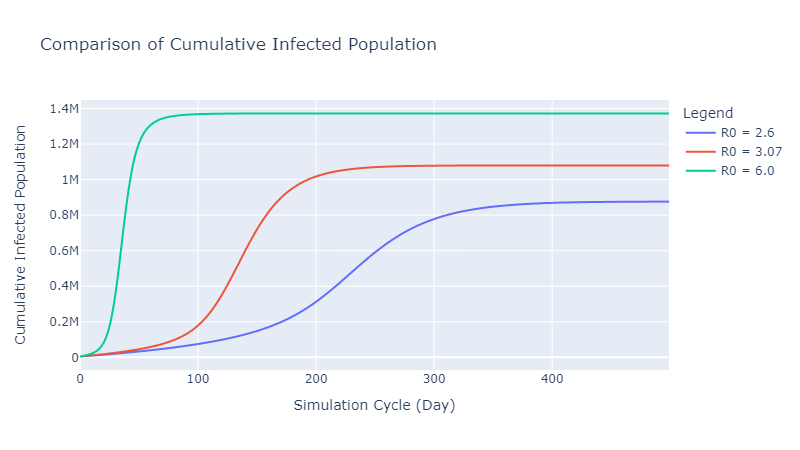
\includegraphics[width=\linewidth]{fig/res-health/InfectedR0.png}
    \caption{Cumulative infected population for $R_0=2.6$, $3.07$, and $6.0$.}
    \label{fig:epidemic_r0}
\end{subfigure}

\vspace{0.5em}

\begin{subfigure}{0.96\textwidth}
    \centering
    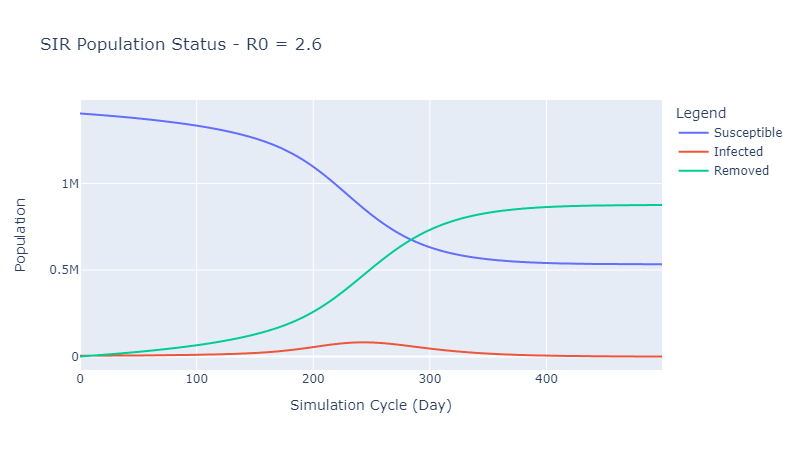
\includegraphics[width=\linewidth]{fig/res-health/SIRPopulationStatus.png}
    \caption{Susceptible, infected, and removed populations over time for the $R_0=2.6$ reference configuration.}
    \label{fig:epidemic_sir_status}
\end{subfigure}

\caption{Epidemic progression under the neighborhood-level configuration. Panel (a) compares cumulative infections under different basic reproduction numbers, while panel (b) shows the population occupying each SIR state for the $R_0=2.6$ reference. Cumulative infections and the population currently infected represent distinct measures of epidemic progression.}
\label{fig:epidemic_transmission_dynamics}
\end{figure}

These results establish two complementary effects of the infection configuration. The cumulative trajectories show the sensitivity of epidemic progression to the configured transmission intensity, while the SIR trajectory illustrates how cumulative incidence differs from the number of individuals simultaneously infected. The $R_0=2.6$ configuration provides the common reference used in the following intervention experiments.


\subsubsection{Vaccination Schedules}
\label{sec:results_epidemic_vaccination}

The second experiment examines vaccination while holding the epidemic configuration at $R_0=2.6$. Daily vaccination quantities follow the Porto Alegre vaccination series described in Section~\ref{sec:vaccination_plugin_inputs} and are distributed among the modeled regions in proportion to their populations. Four vaccination configurations are considered. Configurations A--C introduce progressively larger numbers of doses and associated effectiveness values, while Vaccination D represents an intentionally idealized single-dose configuration with complete modeled effectiveness.

Table~\ref{tbl:epidemic_vaccination_results} summarizes the dose schedules together with the cumulative infection total recorded for each published run. The unvaccinated $R_0=2.6$ simulation is included as the common reference.

\begin{table}[ht]
\centering
\setlength{\tabcolsep}{5pt}
\caption{Published vaccination configurations and cumulative infection outcomes for $R_0=2.6$. Effectiveness values correspond to the modeled reduction in susceptible-to-infected transitions associated with each vaccination level.}
\label{tbl:epidemic_vaccination_results}
\begin{tabularx}{\linewidth}{@{}lcp{3.2cm}p{2.4cm}X@{}}
\toprule
\textbf{Configuration} &
\textbf{Doses} &
\textbf{Effectiveness by dose} &
\textbf{Starting days} &
\textbf{Cumulative infections} \\
\midrule

No vaccination
& 0
& --
& --
& 875,962 \\

Vaccination A
& 1
& 0.4
& 50
& 440,569 \\

Vaccination B
& 2
& 0.4, 0.7
& 50, 150
& 360,607 \\

Vaccination C
& 3
& 0.4, 0.7, 1.0
& 50, 150, 250
& 355,124 \\

Vaccination D
& 1
& 1.0
& 50
& 170,978 \\

\bottomrule
\end{tabularx}
\end{table}

Figure~\ref{fig:epidemic_vaccination} shows how these differences accumulate over time. Even the single-dose Vaccination A configuration substantially reduces cumulative infections relative to the unvaccinated reference, from 875,962 to 440,569. Introducing the second dose in Vaccination B further reduces the total to 360,607. Vaccination C reaches a similar final value of 355,124, while the idealized Vaccination D configuration produces the lowest cumulative total, with 170,978 infections.

The temporal trajectories are particularly informative for Vaccination B and Vaccination C. Both configurations use the same effectiveness values and starting days for their first two doses and therefore remain similar during the initial portion of the simulation. Their configurations diverge when the third dose of Vaccination C begins on day 250. The resulting difference in final cumulative infections is comparatively small relative to the reduction already produced by the first two vaccination levels. This comparison should therefore be interpreted as a difference between complete vaccination schedules rather than as an isolated estimate of the effect of an additional dose.

\begin{figure}[!ht]
\centering
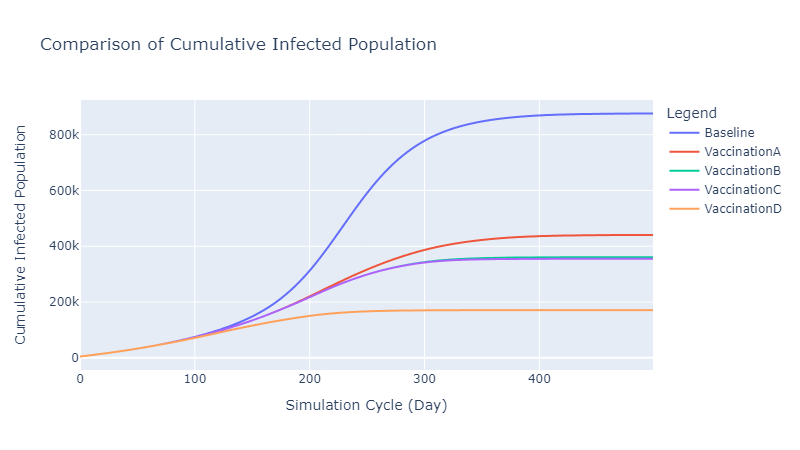
\includegraphics[width=0.96\linewidth]{fig/res-health/InfectedVaccines.png}
\caption{Cumulative infected population under the unvaccinated $R_0=2.6$ reference and Vaccination A--D configurations. The schedules vary in the number of doses, their modeled effectiveness, and their starting days, as summarized in Table~\ref{tbl:epidemic_vaccination_results}.}
\label{fig:epidemic_vaccination}
\end{figure}

Vaccination D provides a useful upper-bound comparison within the implemented behavior, but its effectiveness of 1.0 after a single dose is intentionally idealized. Vaccination C is therefore used instead in the following combined-intervention experiment, since its progressive three-dose schedule provides a less idealized configuration for examining vaccination together with changes in mobility.


\subsubsection{Vaccination and Movement Restriction}
\label{sec:results_epidemic_vaccination_restriction}

The final epidemic experiment examines the combined effect of vaccination and reduced normal-life movement. The epidemic configuration remains fixed at $R_0=2.6$, while movement restriction is varied among 0, 0.50, and 0.75. As described in Section~\ref{sec:levy_walk_plugin_inputs}, the restriction parameter reduces the population selected for the affected routine movements rather than modifying the epidemiological parameters directly. Each restriction value is evaluated both without vaccination and with Vaccination C, producing six configurations.

Figure~\ref{fig:epidemic_vaccination_restriction} presents the cumulative infection trajectories. Relative to the unrestricted and unvaccinated reference, increasing movement restriction reduces the progression of cumulative infections. Vaccination C produces a larger reduction than movement restriction alone, while combining vaccination with stronger movement reduction produces the lowest infection totals.

The strongest combined configuration uses Vaccination C together with a movement restriction of 0.75. This run reaches 140,941 cumulative infections, compared with 875,962 in the unrestricted and unvaccinated reference. This corresponds to an 83.91\% reduction in cumulative infections under the evaluated configuration.

\begin{figure}[ht]
\centering
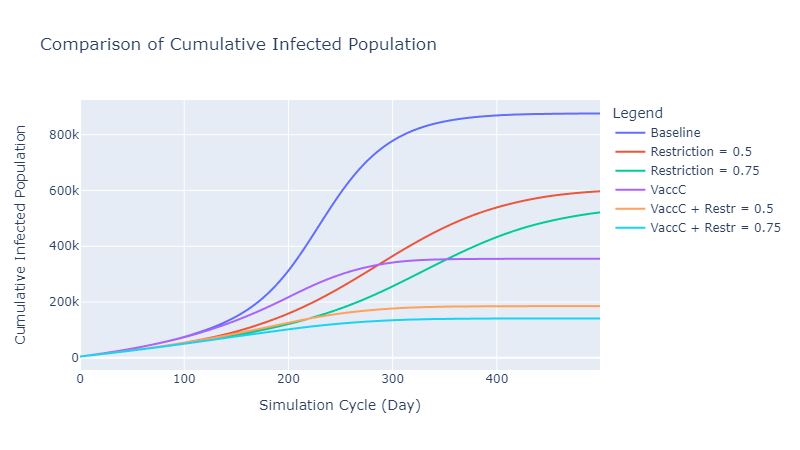
\includegraphics[width=0.96\linewidth]{fig/res-health/InfectedVaccineRestriction.png}
\caption{Cumulative infected population for combinations of movement restriction and Vaccination C under $R_0=2.6$. Restriction values of 0, 0.50, and 0.75 are evaluated both without vaccination and with the three-dose Vaccination C configuration.}
\label{fig:epidemic_vaccination_restriction}
\end{figure}

Taken together, the epidemic experiments show how the same population and mobility configuration can be combined with evolving health states and progressively different intervention conditions. Increasing the configured transmission intensity accelerates epidemic progression, while vaccination and reduced movement both lower cumulative infections under the evaluated scenarios. Their combination produces the lowest reported outcome among the non-idealized intervention configurations.

These results should be interpreted as controlled comparisons among configured epidemic scenarios rather than forecasts of COVID-19 transmission in Porto Alegre. The infection mechanism assumes homogeneous SIR parameters within each configuration and local mixing among populations sharing a POI, while vaccine effectiveness and movement reduction are scenario-defined inputs.

\subsection{Dialysis Access and Infrastructure Resilience}
\label{sec:results_dialysis}

The second health-related application examines access to dialysis as a recurring, capacity-constrained service. In contrast to the epidemic experiments, where the principal outcome is a change in population health state, these simulations evaluate whether scheduled treatment demand can be served by a spatially distributed network of clinics whose availability may depend on supporting infrastructure.

The dialysis behavior, infrastructure dependencies, and disruption inputs are described in Section~\ref{sec:dialysis_plugin_inputs} and Section~\ref{sec:dependency_mapping_plugin_inputs}.
Here, the analysis focuses on treatment completion, waiting, unresolved demand, and travel distance under different service and disruption conditions.

All core scenarios cover ten simulated days, with 24 hourly steps per day. Selected patients require treatment every three days, with initial due days distributed across the treatment interval. When treatment becomes due, patients are assigned to the nearest eligible clinic with available capacity; demand that cannot be admitted remains pending and is reconsidered during subsequent hours.

Clinic operating schedules and treatment capacities are modeled as scenario-defined parameters. By default, clinics operate from 06:00 to 18:00 and admit at most two patients per hour. The exceptions are Centro de Diálise e Transplante and Hospital Moinhos de Vento, which operate until 22:00 and admit at most eight and six patients per hour, respectively.

Two census-sector environments are considered. The reduced environment contains 13 regions, 435 residential POIs, 8 dialysis clinics, and 2 water treatment facilities, while the complete environment contains 94 regions, 2,711 residential POIs, 12 clinics, and 6 water treatment facilities. The reference demand level is configured at 50\% of the nominal three-day treatment capacity of each environment, corresponding to 552 patients in the reduced environment and 696 in the complete environment. Controlled disruptions begin at simulation step 78, corresponding to 06:00 on the third simulated day.
Each reported scenario was executed 30 times. Table~\ref{tbl:dialysis_scenarios} summarizes the configurations used in the comparisons. 

\begin{table}[ht]
\centering
\footnotesize
\setlength{\tabcolsep}{4pt}
\caption{Dialysis scenarios and principal configured conditions.}
\label{tbl:dialysis_scenarios}
\begin{tabularx}{\linewidth}{@{}llrX@{}}
\toprule
\textbf{ID} &
\textbf{Environment} &
\textbf{Patients} &
\textbf{Configured condition} \\
\midrule

D01 & Reduced & 552
& Reference demand level, corresponding to 50\% of nominal three-day capacity. \\

D02 & Reduced  & 552
& ETA Moinhos de Vento is disabled at step 78 and remains unavailable. \\

D03 & Reduced  & 552
& The same ETA is disabled at step 78 and restored four hours later. \\

D04 & Reduced  & 552
& Historical water levels directly affect exposed clinics and water treatment facilities. \\

D05 & Reduced  & 552
& A synthetic 10.1~m water level affects water treatment facilities; clinic unavailability propagates through POI dependencies. \\

D06 & Reduced  & 552
& The scheduled ETA Moinhos outage is combined with a synthetic 9.3~m water-level disruption. \\

D07 & Reduced  & 1,380
& Treatment demand is increased to 125\% of nominal three-day capacity without facility disruption. \\

D08 & Reduced  & 552
& One high-capacity clinic is disabled, removing 128 daily treatment slots. \\

D09 & Reduced  & 552
& Four lower-capacity clinics are disabled, also removing 128 daily treatment slots. \\

D10 & Complete & 696
& Complete-environment reference at 50\% of nominal three-day capacity. \\

D11 & Complete & 696
& Synthetic 9.3~m exposure affects clinics and water sources and is combined with the scheduled ETA Moinhos outage. \\

\bottomrule
\end{tabularx}
\end{table}

Table~\ref{tbl:dialysis_results} provides an overview of the mean outcomes across the 30 repeated executions. Coverage represents the proportion of treatment sessions that become due during the simulation and are completed within the ten-day horizon. Waiting is reported as accumulated due-wait patient-hours, thereby accounting for both the number of patients awaiting treatment and the duration of their wait. Overdue sessions are those that remain due at the end of the simulation. Disabled clinic-hours account only for periods of facility unavailability caused by direct or dependency-related disruptions, rather than ordinary closing hours or exhausted treatment capacity. Distance reports the mean geographic distance from the patient origin to the clinic for admitted treatment sessions.

\begin{table}[ht]
\centering
\footnotesize
\setlength{\tabcolsep}{3pt}
\caption{Mean dialysis outcomes across 30 executions.}
\label{tbl:dialysis_results}
\begin{tabularx}{\linewidth}{
    @{}
    l
    >{\raggedright\arraybackslash}X
    rrrrr
    @{}
}
\toprule
\textbf{ID} &
\textbf{Condition} &
\shortstack{\textbf{Coverage}\\\textbf{(\%)}} &
\shortstack{\textbf{Wait}\\\textbf{(patient-h)}} &
\shortstack{\textbf{Overdue}\\\textbf{(sessions)}} &
\shortstack{\textbf{Disabled}\\\textbf{(clinic-h)}} &
\shortstack{\textbf{Distance}\\\textbf{(km)}} \\
\midrule

D01 & Reduced reference demand
    & 100.00 & 16,640 &   0.0 &     0 & 1.836 \\

D02 & Persistent ETA outage
    &  68.52 & 67,608 & 363.5 &   972 & 2.090 \\

D03 & Four-hour ETA outage
    & 100.00 & 17,238 &   0.0 &    24 & 1.838 \\

D04 & Historical direct flood exposure
    & 100.00 & 17,144 &   0.0 &   225 & 1.768 \\

D05 & Synthetic ETA exposure
    &  50.00 & 84,480 & 552.0 & 1,296 & 1.845 \\

D06 & Combined water and ETA disruption
    &  50.00 & 84,480 & 552.0 & 1,296 & 1.845 \\

D07 & Demand above nominal capacity
    &  93.02 & 106,416 & 114.2 &     0 & 1.854 \\

D08 & One high-capacity clinic unavailable
    & 100.00 & 18,670 &   0.0 &   162 & 1.768 \\

D09 & Four lower-capacity clinics unavailable
    & 100.00 & 18,670 &   0.0 &   648 & 2.037 \\

D10 & Complete reference demand
    & 100.00 & 20,700 &   0.0 &     0 & 6.537 \\

D11 & Complete combined disruption
    &  71.43 & 81,126 & 415.3 & 1,458 & 7.052 \\

\bottomrule
\end{tabularx}
\end{table}

\subsubsection{Service Capacity and Demand Pressure}
\label{sec:results_dialysis_capacity}

The reference scenarios first establish whether the configured clinic networks can serve moderate recurring demand in the absence of disruptions. D01 completes all due treatment sessions in the reduced environment, while D10 likewise reaches 100\% coverage in the complete environment. Nevertheless, the simulations accumulate 16,640 and 20,700 due-wait patient-hours, respectively. Complete treatment coverage therefore does not imply that all patients are treated immediately; waiting provides a complementary measure of service pressure even when all demand can eventually be accommodated.

Scenario D07 isolates the consequence of increased demand without disabling any facility. The number of dialysis patients is increased from 552 to 1,380 in the reduced environment, corresponding to 125\% of the nominal treatment capacity available over a three-day treatment interval. Coverage decreases to 93.02\%, accumulated waiting increases to 106,416 patient-hours, and an average of 114.2 sessions remains overdue at the end of the simulation. In contrast to the infrastructure-disruption scenarios, D07 produces these incomplete treatments with zero disabled clinic-hours. The result therefore distinguishes insufficient available service capacity from failures caused by facility unavailability.
The comparison between D01 and D07 shows the two extremes represented in the simulated scenarios: moderate demand that can be fully absorbed; and demand exceeding the nominal capacity of the reduced network. 

An additional analysis fills the interval between them with demand-to-capacity ratios of 0.25, 0.50, 0.90, 1.00, and 1.25. These correspond to 276, 552, 993, 1,104, and 1,380 patients in the reduced environment and 348, 696, 1,254, 1,392, and 1,740 patients in the complete environment.
Figure~\ref{fig:dialysis_demand_sensitivity} shows that both environments retain 100\% coverage through a demand-to-capacity ratio of 1.00, although accumulated waiting rises continuously. In the reduced environment, mean waiting increases from 6,720 patient-hours at a ratio of 0.25 to 46,800 at 1.00; the corresponding values for the complete environment are 8,400 and 57,840 patient-hours. The sharpest change occurs between ratios 1.00 and 1.25. At 1.25, coverage falls to 93.02\% in both environments, while waiting reaches 106,416 patient-hours in the reduced environment and 133,008 in the complete environment.

\begin{figure}[ht]
    \centering
    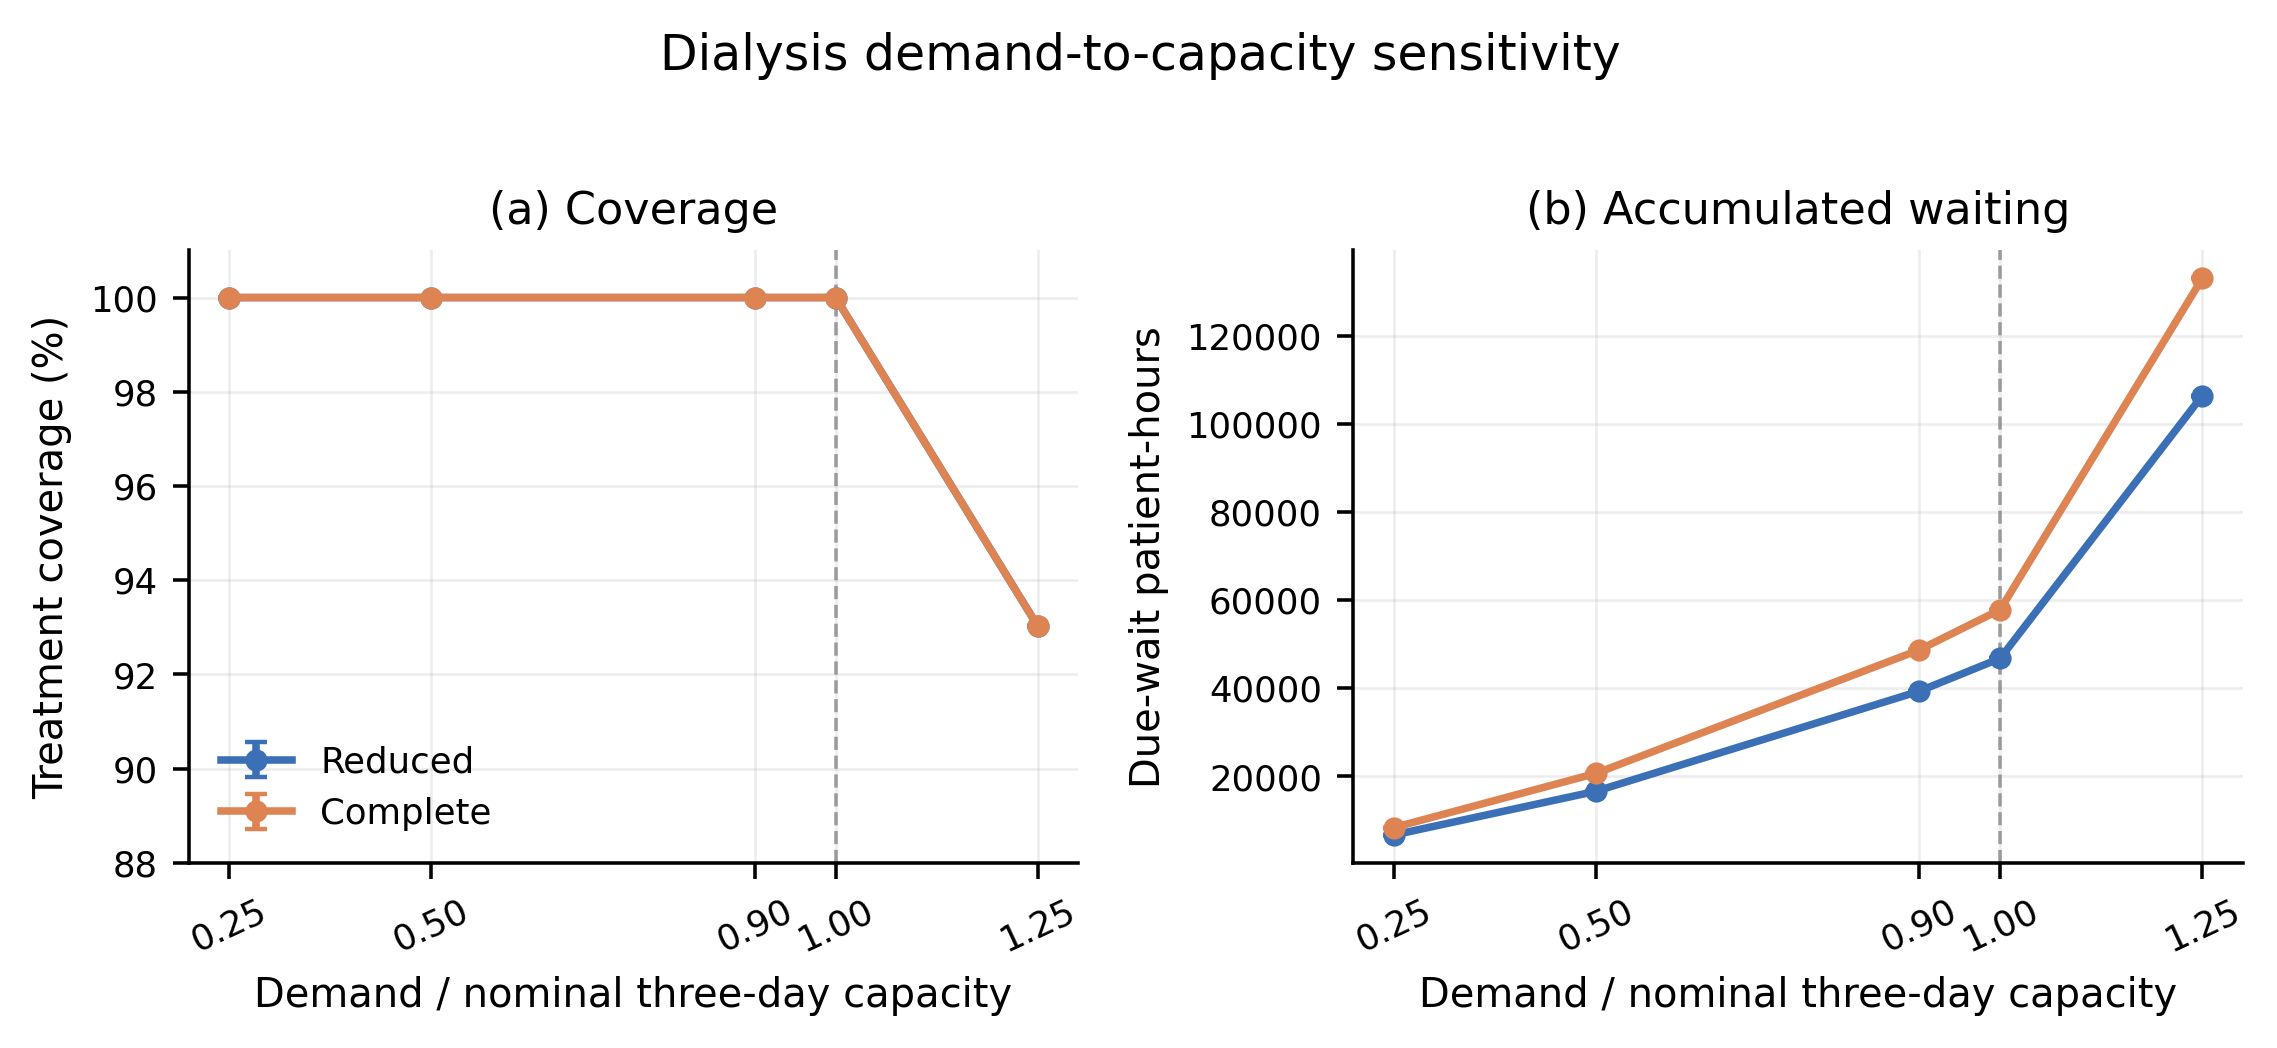
\includegraphics[width=\linewidth]
      {fig/res-health/dialysis_demand_sensitivity.png}
    \caption{Treatment coverage and accumulated waiting under increasing dialysis demand in the reduced and complete census-sector environments. Points show means over 30 simulation executions.}
    \label{fig:dialysis_demand_sensitivity}
\end{figure}


\subsubsection{Infrastructure Disruption and Recovery}
\label{sec:results_dialysis_disruption}

The next scenarios evaluate how service outcomes change when clinic availability is reduced directly or through supporting water infrastructure. D02 and D03 provide the clearest comparison because they begin from the same reduced-environment configuration and apply the same ETA Moinhos de Vento outage at 06:00 on day 3, differing only in whether the facility remains unavailable.

Under the persistent outage in D02, treatment coverage decreases from 100\% in D01 to 68.52\%. Accumulated waiting increases from 16,640 to 67,608 patient-hours, and an average of 363.5 treatment sessions remains overdue at the end of the simulation. The disruption accounts for 972 disabled clinic-hours because clinics dependent on the unavailable ETA remain inaccessible throughout the remaining simulation period.

By contrast, restoring ETA Moinhos de Vento four hours after the initial disruption in D03 is sufficient for all due treatments to be completed within the simulation horizon. Waiting increases only moderately relative to D01, from 16,640 to 17,238 patient-hours, and no sessions remain overdue at the end of the simulation. The comparison therefore shows that the duration of an infrastructure interruption can be more consequential than its occurrence alone: a short interruption creates temporary service pressure, whereas the persistent loss generates a backlog that cannot be cleared within the evaluated period.

The aggregate values, however, do not show how this backlog develops or how quickly service recovers after restoration. Figure~\ref{fig:dialysis_outage_recovery} aligns the hourly response across the 30 simulation runs. The outage begins at step 78 and the D03 restoration occurs at step 82, four hours later. During this interval, available treatment capacity in D03 falls from 26 to 4 slots per hour. After restoration, the number of patients with treatment due and still waiting returns to the D01 level at step 88, six hours after restoration, and cumulative treatment completions catch up with D01 at step 89. In D02, by contrast, only four slots per hour remain available during clinic opening periods after the disruption, so the backlog persists to the end of the simulation.

\begin{figure}[ht]
    \centering
    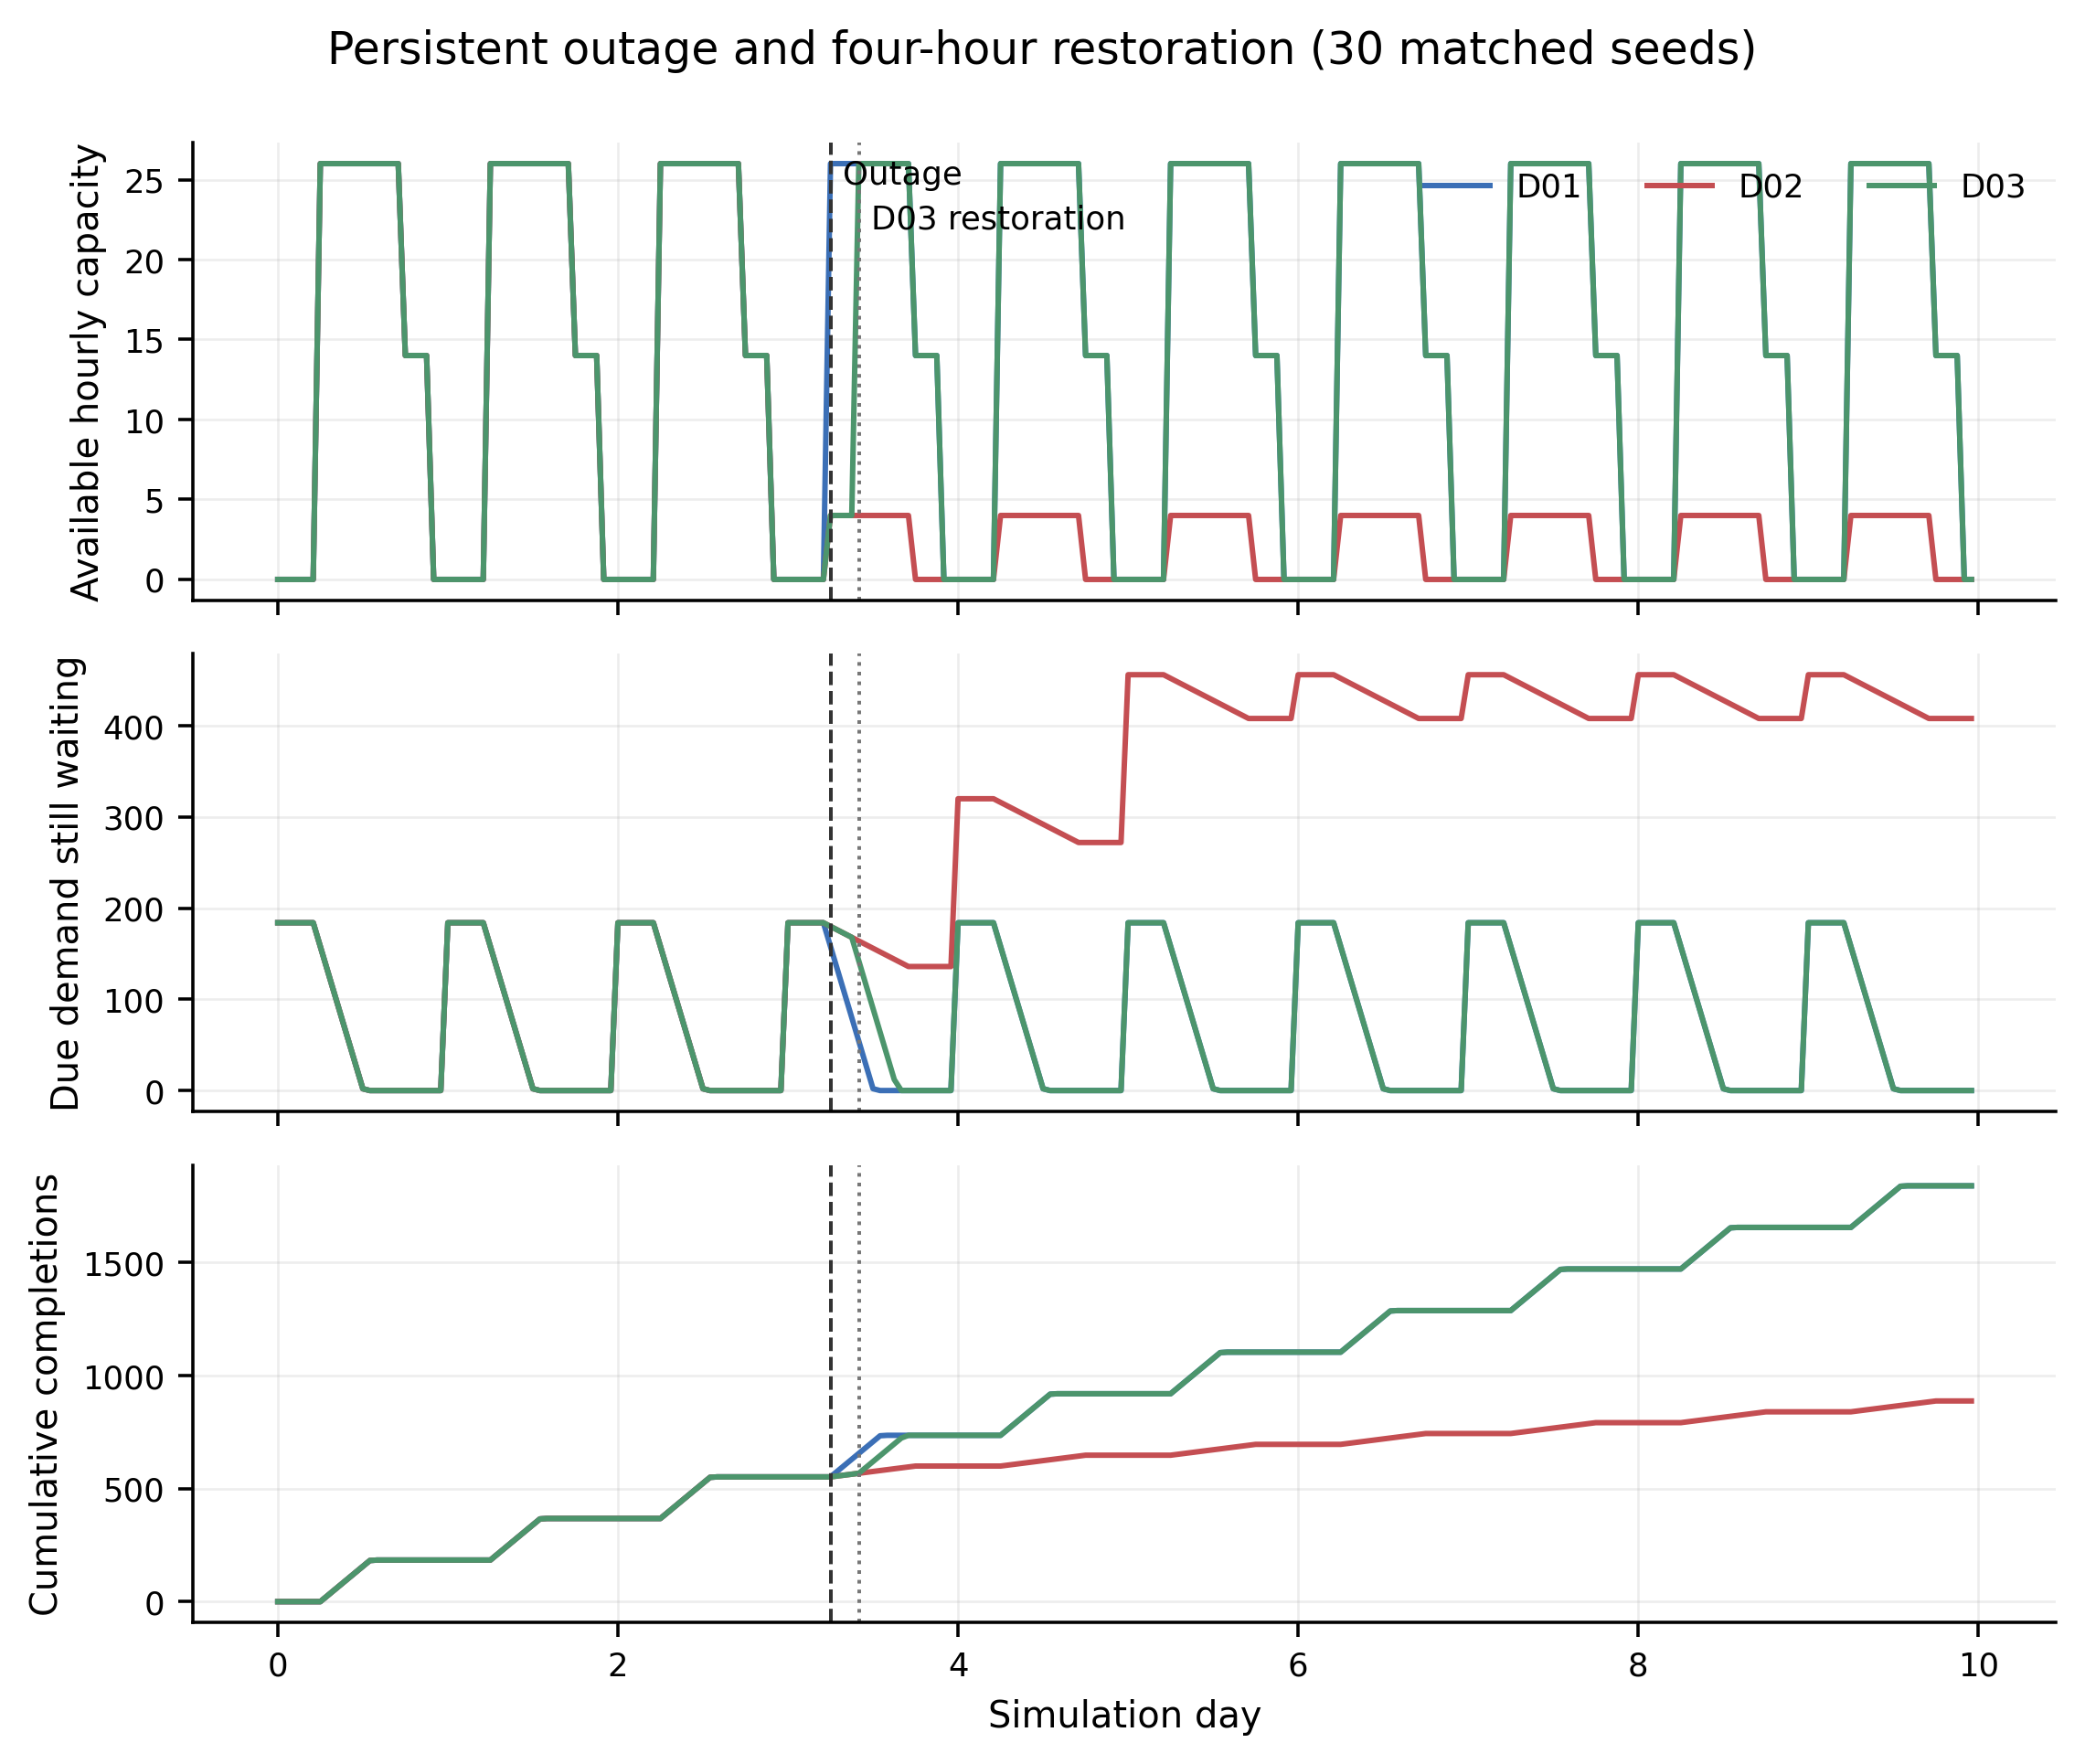
\includegraphics[width=\linewidth]
      {fig/res-health/dialysis_outage_recovery_d01_d02_d03.png}
    \caption{Mean hourly treatment response over 30 matched seeds for the reference (D01), persistent outage (D02), and temporary outage (D03) scenarios. Vertical markers identify the disruption and restoration steps.}
    \label{fig:dialysis_outage_recovery}
\end{figure}

Scenarios D04--D06 extend the comparison to flood-related and dependency disruptions. D04 applies the historical water-level series directly to the exposure thresholds of clinics and water treatment facilities. Although this produces 225 disabled clinic-hours, the network retains 100\% treatment coverage and accumulates 17,144 patient-hours of waiting, only 504 more than the D01 reference. In this configuration, the temporary facility losses can therefore be absorbed by the remaining service network within the ten-day simulation.

D05 instead applies a synthetic 10.1~m water level only to water treatment facilities, allowing clinic unavailability to propagate through the configured POI dependencies. This produces a substantially stronger effect: coverage falls to 50\%, accumulated waiting reaches 84,480 patient-hours, and an average of 552 treatment sessions remains overdue. The scenario accumulates 1,296 disabled clinic-hours.

D06 combines a scheduled ETA Moinhos outage with a synthetic 9.3~m water-level disruption and produces the same aggregate outcomes as D05: 50\% coverage, 84,480 patient-hours of waiting, 552 overdue sessions, and 1,296 disabled clinic-hours. These results show that the identical service outcomes arise through different direct mechanisms. In D05, flood blockers affect both the Menino Deus and Moinhos de Vento water sources. In D06, flooding blocks Menino Deus while the scheduled outage blocks Moinhos de Vento. In both cases, dependency conditions consequently disable all eight clinics. Thus, the infrastructure-level causes differ, but they yield the same effective clinic availability and aggregate treatment outcomes.

The complete census-sector environment provides an additional comparison at a larger spatial scale. D10 serves as its moderate reference demand and completes all due treatment sessions, with 20,700 accumulated patient-hours of waiting. Under the combined disruption in D11, coverage decreases to 71.43\%, accumulated waiting rises to 81,126 patient-hours, and an average of 415.3 sessions remains overdue. Mean admission distance also increases from 6.537~km to 7.052~km.

Across the 30 simulation run, D11 adds 60,426 patient-hours of waiting and 0.516~km to the mean admission distance relative to D10. The availability of a larger clinic network does not prevent substantial service loss under the evaluated geographically distributed disruption. This comparison should not, however, be interpreted as an isolated effect of increasing environment size, because the reduced and complete environments also differ in patient counts, clinic locations, water sources, and dependency structure.


\subsubsection{Spatial Consequences of Clinic Failure}
\label{sec:results_dialysis_spatial}

The final comparison examines whether the spatial distribution of unavailable treatment capacity affects service access. D08 and D09 remove the same nominal amount of service, 128 treatment slots per day, but distribute this loss differently across the reduced network. D08 disables one high-capacity clinic, whereas D09 disables four lower-capacity clinics.

Both scenarios maintain 100\% treatment coverage and produce the same accumulated waiting of 18,670 patient-hours. Consequently, the two failure patterns are equivalent with respect to these aggregate service outcomes under the configured demand. Their spatial effects, however, differ. Mean admission distance is 1.768~km in D08 and 2.037~km in D09, corresponding to an increase of 0.269~km when the same capacity loss is distributed across four clinics.

D09 also accumulates more disabled clinic-hours, 648 compared with 162 in D08, because the same removed capacity is distributed across a larger number of facilities. Disabled clinic-hours should therefore not be interpreted as an alternative measure of lost treatment capacity in this comparison: the scenarios intentionally remove the same nominal daily capacity but differ in the number of facilities over which that loss occurs.

The increase in mean admission distance indicates that capacity alone does not fully describe the effect of clinic loss. When multiple facilities are removed from different locations, patients who can still be treated may need to travel farther through the remaining service network. D08 and D09 therefore provide a controlled comparison in which treatment completion is preserved while the spatial cost of accessing treatment increases.


Taken together, the dialysis experiments distinguish several sources of service pressure. High demand can produce incomplete treatment without any facility becoming unavailable, while infrastructure disruptions can reduce effective service capacity even under otherwise moderate demand. Temporary and persistent failures produce substantially different outcomes, and equal nominal capacity losses can generate different travel requirements depending on which clinics become unavailable.

These results also show why dialysis-service performance cannot be characterized by coverage alone. Accumulated waiting captures delays that remain hidden when all treatments are eventually completed, overdue demand identifies sessions that cannot be recovered within the simulation horizon, and travel distance reflects the spatial consequence of redistribution across the clinic network.

The results remain conditional on the implemented service assumptions. Patients are assigned to the nearest eligible clinic with available capacity, treatment occupies one simulation step, and untreated demand is reconsidered in later hours. Appointment priorities, clinical deterioration, hospitalization, mortality, and other consequences of delayed treatment are not represented. Similarly, clinic capacities, disruption schedules, infrastructure dependencies, and synthetic water levels are scenario inputs. The experiments therefore support controlled comparisons of service behavior under the evaluated configurations rather than predictions of dialysis accessibility during an actual disruption in Porto Alegre.

\subsection{Main Findings}
\label{sec:health_results_findings}

The experiments in this section extend the mobility-oriented analyses of the preceding sections by considering scenarios in which population movement interacts with health states and access to recurring services. The epidemic experiments examine how mobility contributes to the evolution of infection across the population, whereas the dialysis experiments examine how mobility determines access to a spatially distributed and capacity-constrained healthcare network. Together, they demonstrate two complementary ways in which population movement can influence health-related outcomes.

The epidemic experiments show that changes in the configured transmission intensity substantially alter the progression of infection while preserving the same population and mobility configuration. Vaccination and reduced routine movement both decrease cumulative infections under the evaluated scenarios, and their combination produces the strongest reduction among the non-idealized intervention configurations. These results also illustrate the distinction between cumulative infection and the population simultaneously occupying the infected state, allowing different aspects of epidemic progression to be examined within the same population representation.

The dialysis experiments demonstrate that treatment access depends not only on the amount of nominal service capacity but also on when and where that capacity is available. Increasing demand progressively raises waiting even while all due treatments can still be completed, with incomplete treatment emerging once demand exceeds the configured nominal capacity. Infrastructure disruptions produce a different form of service loss: temporary outages may be absorbed by the remaining network, whereas persistent or geographically distributed disruptions can generate substantial unresolved treatment demand.

The dialysis results further show that service performance cannot be characterized by treatment coverage alone. Waiting identifies service pressure before incomplete treatment occurs, overdue sessions indicate demand that cannot be recovered within the simulation horizon, and admission distance captures changes in spatial access when patients are redistributed among available clinics. Similarly, failures removing the same nominal treatment capacity can preserve the same coverage and waiting while producing different travel requirements depending on which facilities become unavailable.

Overall, these experiments show how the population representation can support processes whose outcomes extend beyond movement itself. Mobility determines opportunities for interaction in the epidemic scenarios and access to available services in the dialysis scenarios, while additional state, capacity, and dependency constraints determine the resulting health-related outcomes. The experiments therefore complement the preceding mobility and disruption analyses by demonstrating how the same simulation framework can represent interactions between population movement, evolving individual states, recurring service demand, and infrastructure availability.